\documentclass[12pt,a4paper,reqno]{amsart}

% language
\usepackage[greek,english]{babel}
\usepackage[utf8]{inputenc}
\usepackage{alphabeta}

% change default names to greek
\addto\captionsenglish{
    \renewcommand{\contentsname}{Περιεχόμενα}
    \renewcommand{\refname}{Βιβλιογραφία}
    \renewcommand{\datename}{Ημερομηνία:}
    \renewcommand{\urladdrname}{Ιστοσελίδα}
}

% math 
\usepackage{amsmath,amsthm,amssymb,amscd}

% font
\usepackage[cal=euler]{mathalfa}
\usepackage{libertinus-type1}
% \usepackage{txfonts} % for upright greek letters
\usepackage{bm} % for bold symbols
\usepackage{bbm} % for the simply-looking bb symbols

% miscellaneous 
\usepackage{changepage} %for indenting environments
\usepackage{csquotes} % example: \textcquote{}
\usepackage{blkarray}
\setcounter{MaxMatrixCols}{20} % default for pmatrix is 10!!
\usepackage{ytableau}

% drawing
\usepackage{tikz,tikz-cd}
\usetikzlibrary{shapes.misc, patterns, matrix, calc, intersections,positioning}
\usepackage{graphics,graphicx}
\usepackage{float} % provides enhanced control and customization options for floating objects such as figures and tables

% colors
\usepackage{xcolor}
\definecolor{darkcandyapplered}{rgb}{0.64, 0.0, 0.0}
\definecolor{midnightblue}{rgb}{0.1, 0.1, 0.44}
\definecolor{mylightblue}{HTML}{336699}
\definecolor{burntorange}{rgb}{0.8, 0.33, 0.0}
\definecolor{iceberg}{rgb}{0.44, 0.65, 0.82}
\definecolor{applegreen}{rgb}{0.55, 0.71, 0.0}
\definecolor{canaryyellow}{rgb}{1.0, 0.94, 0.0}

% hrefs
\usepackage{hyperref}
\usepackage[noabbrev,capitalize]{cleveref}
\hypersetup{
    pdftoolbar=true,        
    pdfmenubar=true,        
    pdffitwindow=false,     
    pdfstartview={FitH},  % fits the width of the page to the window
    pdftitle={},
    pdfauthor={},
    pdfsubject={},
    pdfkeywords={},
    pdfnewwindow=true,  % links in new window
    colorlinks=true,  % false: boxed links; true: colored links
    linkcolor=darkcandyapplered,   % color of internal links
    citecolor=midnightblue,  % color of links to bibliography
    urlcolor=cyan,  % color of external links
    linktocpage=true  % changes the links from the section body to the page number
    }

% geometry
\textwidth=16cm 
\textheight=21cm 
\hoffset=-55pt 
\footskip=25pt

% thm envs (you might need to change the path)
% In this macro I define all the theorem environments

\theoremstyle{definition}
\newtheorem{theorem}{Θεώρημα}
\newtheorem{proposition}[theorem]{Πρόταση}
\newtheorem{lemma}[theorem]{Λήμμα}
\newtheorem{corollary}[theorem]{Πόρισμα}
\newtheorem{conjecture}[theorem]{Εικασία}
\newtheorem{problem}[theorem]{Πρόβλημα}
\newtheorem*{claim}{Ισχυρισμός}
\newtheorem{observation}[theorem]{Παρατήρηση}
\newtheorem{definition}[theorem]{Ορισμός}
\newtheorem{question}[theorem]{Ερώτηση}
\newtheorem*{questions}{Ερωτήματα}
\newtheorem{example}[theorem]{Παράδειγμα}
\newtheorem{exercise}{Άσκηση}

\newtheorem*{combInterlude}{Ιντερλούδιο Συνδυαστικής}
\newtheorem*{example_cont}{Παράδειγμα~6.6}
\newtheorem*{digression_la}{Παρέκβαση Γραμμικής Άλγεβρας}
\newtheorem*{thm}{Θεώρημα}

\theoremstyle{remark}
\newtheorem*{remark}{Παρατήρηση}

% fixes the correct numbering of environments
\numberwithin{theorem}{section}
\numberwithin{exercise}{section}
\numberwithin{equation}{section}

% math ops (you might need to change the path)
% In this macro I define all of my math operators

% fields
\newcommand{\NN}{\mathbbmss{N}} 
\newcommand{\ZZ}{\mathbbmss{Z}} 
\newcommand{\QQ}{\mathbbmss{Q}} 
\newcommand{\RR}{\mathbbmss{R}} 
\newcommand{\CC}{\mathbbmss{C}} 
\newcommand{\KK}{\mathbbmss{K}} 
\newcommand{\FF}{\mathbbmss{F}} 

% symmetric group
\newcommand{\fS}{\mathfrak{S}}  

% calligraphic 
\newcommand{\aA}{\mathcal{A}} 
\newcommand{\bB}{\mathcal{B}}
\newcommand{\cC}{\mathcal{C}}
\newcommand{\dD}{\mathcal{D}}
\newcommand{\eE}{\mathcal{E}}
\newcommand{\fF}{\mathcal{F}}
\newcommand{\hH}{\mathcal{H}}
\newcommand{\iI}{\mathcal{I}}
\newcommand{\lL}{\mathcal{L}}
\newcommand{\oO}{\mathcal{O}}
\newcommand{\pP}{\mathcal{P}}
\newcommand{\sS}{\mathcal{S}}
\newcommand{\mM}{\mathcal{M}}
\newcommand{\uU}{\mathcal{U}}

% bold
\newcommand{\bfa}{\mathbf{a}}
\newcommand{\bfe}{\mathbf{e}}
\newcommand{\bfF}{\pmb{F}}
\newcommand{\bfR}{\pmb{R}}
\newcommand{\bfv}{\mathbf{v}}
%\newcommand{\bfx}{\bm{x}}
%\newcommand{\bfx}{\mathbf{x}} 
\newcommand{\bfx}{\pmb{x}}
\newcommand{\bfX}{\pmb{X}}
\newcommand{\bfy}{\pmb{y}}
\newcommand{\bfz}{\pmb{z}}

% roman
\newcommand{\rmA}{\mathrm{A}}
\newcommand{\rmB}{\mathrm{B}}
\newcommand{\rmC}{\mathrm{C}}
\newcommand{\rmD}{\mathrm{D}} 
\newcommand{\rmI}{\mathrm{I}} 
\newcommand{\rmK}{\mathrm{K}}
\newcommand{\rmM}{\mathrm{M}}
\newcommand{\rmP}{\mathrm{P}}  
\newcommand{\rmp}{\mathrm{p}}  
\newcommand{\rmQ}{\mathrm{Q}}  
\newcommand{\rmR}{\mathrm{R}}
\newcommand{\rmS}{\mathrm{S}}
\newcommand{\rmT}{\mathrm{T}}
\newcommand{\rmU}{\mathrm{U}}
\newcommand{\rmV}{\mathrm{V}}
\newcommand{\rmY}{\mathrm{Y}}
\newcommand{\rmZ}{\mathrm{Z}}
\newcommand{\rmz}{\mathrm{z}}

% greek letters
% I'm renewing some commands in order to appear in upright font
% If I want to change it later, I don't have to do it manually, I just change it from here.
% \newcommand{\uaa}{\alphaup}
% \renewcommand{\alpha}{\alphaup}
% \renewcommand{\beta}{\betaup}
% \renewcommand{\gamma}{\gammaup}
% \renewcommand{\delta}{\deltaup}
% \renewcommand{\epsilon}{\epsilonup}
% \newcommand{\ee}{\epsilon}
% \renewcommand{\varepsilon}{\varepsilonup}
% \renewcommand{\theta}{\thetaup}
% \renewcommand{\lambda}{\lambdaup}
% \newcommand{\ull}{\lambda}
% \renewcommand{\mu}{\muup}
% \renewcommand{\nu}{\nuup}
% \renewcommand{\pi}{\piup}
% \renewcommand{\rho}{\rhoup}
% \renewcommand{\varrho}{\varrhoup}
% \renewcommand{\sigma}{\sigmaup}
% \renewcommand{\tau}{\tauup} 
% \renewcommand{\phi}{\phiup}
% \renewcommand{\chi}{\chiup}
% \renewcommand{\psi}{\psiup}
% \renewcommand{\omega}{\omegaup}

% arrows and symbols 
\renewcommand{\to}{\rightarrow}
\newcommand{\toto}{\longrightarrow}
\newcommand{\mapstoto}{\longmapsto}
\newcommand{\then}{\Rightarrow}
\newcommand{\IFF}{\Leftrightarrow}
\newcommand{\tl}{\tilde}
\newcommand{\wtl}{\widetilde}
\newcommand{\ol}{\overline}
\newcommand{\ul}{\underline}
\newcommand{\oldemptyset}{\emptyset}
\renewcommand{\emptyset}{\varnothing}
\DeclareMathSymbol{\Arg}{\mathbin}{AMSa}{"39} % for arguments 
\newcommand{\onto}{\ensuremath{\twoheadrightarrow}}
\newcommand{\tle}{\trianglelefteq}
\newcommand{\tge}{\trianglerighteq}

% absolute value symbol
\usepackage{mathtools} 
\DeclarePairedDelimiter\abs{\lvert}{\rvert}%
\DeclarePairedDelimiter\norm{\lVert}{\rVert}%
\makeatletter
\let\oldabs\abs
\def\abs{\@ifstar{\oldabs}{\oldabs*}}

% tensor symbol
\newcommand{\tensor}[1]{%
  \mathbin{\mathop{\otimes}\limits_{#1}}%
}

% permutation cycle notation
\ExplSyntaxOn
\NewDocumentCommand{\cycle}{ O{\;} m }
 {
  (
  \alec_cycle:nn { #1 } { #2 }
  )
 }

\seq_new:N \l_alec_cycle_seq
\cs_new_protected:Npn \alec_cycle:nn #1 #2
 {
  \seq_set_split:Nnn \l_alec_cycle_seq { , } { #2 }
  \seq_use:Nn \l_alec_cycle_seq { #1 }
 }
\ExplSyntaxOff

% setminus symbol
\newcommand{\mysetminusD}{\hbox{\tikz{\draw[line width=0.6pt,line cap=round] (3pt,0) -- (0,6pt);}}}
\newcommand{\mysetminusT}{\mysetminusD}
\newcommand{\mysetminusS}{\hbox{\tikz{\draw[line width=0.45pt,line cap=round] (2pt,0) -- (0,4pt);}}}
\newcommand{\mysetminusSS}{\hbox{\tikz{\draw[line width=0.4pt,line cap=round] (1.5pt,0) -- (0,3pt);}}}
\newcommand{\sm}{\mathbin{\mathchoice{\mysetminusD}{\mysetminusT}{\mysetminusS}{\mysetminusSS}}}

% custom math operators
\newcommand{\Des}{\mathrm{Des}} 
\newcommand{\des}{\mathrm{des}} 
\newcommand{\Asc}{\mathrm{Asc}}
\newcommand{\asc}{\mathrm{asc}} 
\newcommand{\inv}{\mathrm{inv}}
\newcommand{\Inv}{\mathrm{Inv}}
\newcommand{\maj}{\mathrm{maj}} 
\newcommand{\comaj}{\mathrm{comaj}} 
\newcommand{\fix}{\mathrm{fix}} 
\newcommand{\Sym}{\mathrm{Sym}} 
\newcommand{\QSym}{\mathrm{QSym}}
\newcommand{\FQSym}{\mathrm{FQSym}} 
\newcommand{\End}{\mathrm{End}} 
\newcommand{\Rad}{\mathrm{Rad}} 
\newcommand{\rmMat}{\mathrm{Mat}} 
\newcommand{\rmdim}{\mathrm{dim}} 
\newcommand{\rmTop}{\mathrm{Top}} 
\newcommand{\rmCF}{\mathrm{CF}} 
\newcommand{\rmId}{\mathrm{Id}}
\newcommand{\rmid}{\mathrm{id}}
\newcommand{\rmtw}{\mathrm{tw}}
\newcommand{\trace}{\mathrm{tr}}
\newcommand{\Irr}{\mathrm{Irr}}
\newcommand{\Ind}{\mathrm{Ind}} % induction
\newcommand{\Res}{\mathrm{Res}} % restriction
\newcommand{\triv}{\mathrm{triv}} % trivial rep
\newcommand{\rmdef}{\mathrm{def}} % defining rep
\newcommand{\dom}{\triangleleft}
\newcommand{\domeq}{\trianglelefteq}
\newcommand{\lex}{\mathrm{lex}}
\newcommand{\sign}{\mathrm{sign}}
\newcommand{\SYT}{\mathrm{SYT}}
\renewcommand{\Im}{\mathrm{Im}}
\newcommand{\Ker}{\mathrm{Ker}}
\newcommand{\GL}{\mathrm{GL}}
\newcommand{\FL}{\mathrm{FL}}
\newcommand{\Span}{\mathrm{span}}
\newcommand{\pos}{\mathrm{pos}}
\newcommand{\Comp}{\mathrm{Comp}}
\newcommand{\Set}{\mathrm{Set}}
\newcommand{\std}{\mathrm{std}}
\newcommand{\cont}{\mathrm{cont}} %content of a SSYT
\newcommand{\SSYT}{\mathrm{SSYT}}
\newcommand{\ct}{\mathrm{ct}} % cycle type
\newcommand{\ch}{\mathrm{ch}} % Frobenius characteristic map
\newcommand{\height}{\mathrm{ht}}
\newcommand{\FPS}{\CC[\![\bfx]\!]} % formal power series
\newcommand{\FPSS}{\CC[\![\bfx,\bfy]\!]}
\newcommand{\reg}{\mathrm{reg}}
\newcommand{\hook}{\mathrm{h}}
\newcommand{\weight}{\mathrm{wt}}
\newcommand{\co}{\mathrm{co}}
\newcommand{\ps}{\mathrm{ps}}
\newcommand{\rmsum}{\mathrm{sum}}
\newcommand{\NSym}{\mathrm{NSym}}
\newcommand{\Hom}{\mathrm{Hom}}
\newcommand{\proj}{\mathrm{proj}}
\newcommand{\stat}{\mathrm{stat}}
\newcommand{\Par}{\mathrm{Par}}
\newcommand{\rmset}{\mathrm{set}}
\newcommand{\comp}{\mathrm{comp}}

% miscellaneous commands
\newcommand{\defn}[1]{{\color{mylightblue}{#1}}}
\newcommand{\toDo}{{\bf\color{red} TODO}}
\newcommand{\toCite}{{\bf\color{green} CITE}}
\newcommand*{\vertbar}{\rule[-1ex]{0.5pt}{2.5ex}} % for matrices with column vectors
\newcommand*{\horzbar}{\rule[.5ex]{2.5ex}{0.5pt}} % for matrices with row vectors
\newcommand{\myblue}[1]{{\color{iceberg}{#1}}}
\newcommand{\myorange}[1]{{\color{burntorange}{#1}}}
\newcommand{\mygreen}[1]{{\color{applegreen}{#1}}}
\newcommand{\myred}[1]{{\color{darkcandyapplered}{#1}}}

% ferrer's diagram
\newcommand{\fdiagram}[1]{
    \begin{tikzpicture}[scale=.7]
        \fill foreach \Z [count=\Y] in {#1}
        {foreach \X in {1,...,\Z} 
        {(\X,-\Y) circle[radius=3pt]}};
    \end{tikzpicture}
}

%
\newcommand{\tcbo}[1]{\textcolor{burntorange}{#1}}

% 
\newenvironment{nouppercase}{%
  \let\uppercase\relax%
  \renewcommand{\uppercasenonmath}[1]{}}{}

% titlepage
\title{Θ2.04: Θεωρία Αναπαραστάσεων και Συνδυαστική}
\author[Β.~Δ. Μουστακας]{Βασίλης Διονύσης Μουστάκας \\ Πανεπιστήμιο Κρήτης}
\date{25 Νοεμβρίου 2025}
% \urladdr{\href{https://sites.google.com/view/vasmous}{https://sites.google.com/view/vasmous}}

\begin{document}

\begingroup
\def\uppercasenonmath#1{} % this disables uppercase title
\let\MakeUppercase\relax % this disables uppercase authors
\maketitle
\endgroup

\setcounter{section}{11}
\setcounter{theorem}{7}
\begin{center}
    \textbf{11. Πρότυπα Specht
} (Συνέχεια)
\end{center}

\begin{proof}[Απόδειξη του Θεωρήματος 11.5]
    Έστω $\lambda$ μια διαμέριση ακεραίου και $U$ ένα υποπρότυπο του $\rmM^\lambda$. Το Λήμμα 11.7 (4) μας πληροφορεί ότι για κάθε $u \in U$ και κάθε ταμπλώ $T$ σχήματος $\lambda$ ισχύει ότι $\nabla_T^-u = c\,\bfe_T$, για κάποιο $c \in \CC$. Διακρίνουμε περιπτώσεις.

    Αν για κάθε $u \in U$ και κάθε ταμπλώ $T$ σχήματος $\lambda$ ισχύει ότι $c = 0$, τότε 
    \[
    (u, \bfe_T) = (u, \nabla_T^-[T]) = (\nabla_T^-u, [T]) = (0,[T]) = 0,
    \]
    όπου η δεύτερη ισότητα έπεται από το Λήμμα 11.7 (1) και γι αυτό $u \in (\sS^\lambda)^\perp$. Άρα, $U \subseteq (\sS^\lambda)^\perp$.

    Διαφορετικά, υπάρχει κάποιο $u \in U$ και κάποιο ταμπλώ $T$ σχήματος $\lambda$ για τα οποία $c \neq 0$. Τότε 
    \[
    \bfe_T = \frac{1}{c}\nabla_T^-u \ \in U,
    \]
    διότι το $U$ είναι υποπρότυπο του $\rmM^\lambda$. Άρα, $\sS^\lambda \subseteq U$ λόγω της κυκλικότητας του $\sS^\lambda$ και η απόδειξη ολοκληρώνεται.
\end{proof}

Στην απόδειξη του Λήμματος 11.7 (3) είδαμε ότι αν δυο ταμπλώ $T, Q$ ίδιου σχήματος έχουν την ιδιότητα ότι κάθε δυο στοιχεία που ανήκουν στην ίδια γραμμή του $Q$ δεν μπορούν να ανήκουν στην ίδια στήλη του $T$, τότε υπάρχει μια μετάθεση $\pi \in \rmC(T)$ τέτοια ώστε $[\pi{T}] = [Q]$. Τι γίνεται αν τα $T$ και $Q$ έχουν διαφορετικό σχήμα;

Για παράδειγμα, έστω 
\[
    T = 
    \ytableausetup{nosmalltableaux,notabloids,centertableaux}
    \ytableaushort{3786,152,4},
    \quad 
    \text{και}
    \quad
    Q = \ytableaushort{615,42,8,3,7}
\]
δυο ταμπλώ σχήματος $\lambda = (4,3,1)$ και $\mu = (3,2,1,1,1)$ και περιεχομένου $[8]$. Κάνοντας την ίδια διακασία, όπως στην απόδειξη του Λήμματος 11.7 (3), επειδή $\lambda \neq \mu$, δεν μπορούμε να μεταθέσουμε τα στοιχεία κάθε στήλης του $T$ με σκοπό να βρεθούν στην αντίστοιχη θέση που έχουν στις γραμμές του $Q$, αλλά μπορούμε να τα μεταθέσουμε ώστε να βρεθούν στην ίδια \emph{σχετική} σειρά στις γραμμές του $T$ με αυτή που έχουν στις γραμμές του του $Q$. Στο παράδειγμα, στην πρώτη στήλη 
\[
    T = 
    \begin{ytableau}
        *(burntorange)3 & 7 & 8 & 6 \\
        *(burntorange)1 & 5 & 2 \\
        *(burntorange)4 \\
    \end{ytableau}
    \quad 
    \text{και}
    \quad
    Q = 
    \begin{ytableau}
        6 & *(burntorange)1 & 5 \\
        *(burntorange)4 & 2  \\
        8 \\
        *(burntorange)3 \\
        7
    \end{ytableau}
\]
και γι αυτό δρούμε με την $\cycle{1,4,3}$. Έπειτα, για τη δεύτερη στήλη 
\[
    \cycle{1,4,3} T = 
    \begin{ytableau}
        1 & *(iceberg)7 & 8 & 6 \\
        4 & *(iceberg)5 & 2 \\
        3 \\
    \end{ytableau}
    \quad 
    \text{και}
    \quad
    Q = 
    \begin{ytableau}
        6 & 1 & *(iceberg)5 \\
        4 & 2  \\
        8 \\
        3 \\
        *(iceberg)7
    \end{ytableau}
\]
και γι αυτό δρούμε με την $\cycle{5,7}$. Τέλος, για την τρίτη στήλη
\[
    \cycle{5,7}\cycle{1,4,3} T = 
    \begin{ytableau}
        1 & 5 & *(applegreen)8 & 6 \\
        4 & 7 & *(applegreen)2 \\
        3 \\
    \end{ytableau}
    \quad 
    \text{και}
    \quad
    Q = 
    \begin{ytableau}
        6 & 1 & 5 \\
        4 & *(applegreen)2  \\
        *(applegreen)8 \\
        3 \\
        7
    \end{ytableau}
\]
και γι αυτό δρούμε με την $\cycle{2,8}$, για να προκύψουν τα ταμπλώ 
\[
    \cycle{2,8}\cycle{5,7}\cycle{1,4,3} T = 
    \begin{ytableau}
        *(burntorange)1 & *(iceberg)5 & *(applegreen)2 & 6 \\
        *(burntorange)4 & *(iceberg)7 & *(applegreen)8 \\
        *(burntorange)3 \\
    \end{ytableau}
    \quad 
    \text{και}
    \quad
    Q = 
    \begin{ytableau}
        6 & *(burntorange)1 & *(iceberg)5 \\
        *(burntorange)4 & *(applegreen)2  \\
        *(applegreen)8 \\
        *(burntorange)3 \\
        *(iceberg)7
    \end{ytableau}.
\]
Συμπερασματικά, προκύτπει το παρακάτω, το οποίο είναι γνωστό ως το λήμμα κυριαρχίας (dominance lemma) για διαμερίσεις ακεραίων.

\begin{proposition}
    \label{prop:dominance_lemma}
    Έστω $\lambda = (\lambda_1, \lambda_2, \dots)$ και $\mu = (\mu_1, \mu_2, \dots)$ δυο διαμερίσεις ακεραίων. Αν $T$ και $Q$ είναι ταμπλώ σχήματος $\lambda$ και $\mu$, αντίστοιχα, με την ιδιότητα κάθε δυο στοιχεία που ανήκουν στην ίδια γραμμή του $Q$ δεν μπορούν να ανήκουν στην ίδια στήλη του $T$, τότε
    \begin{itemize}
        \item[(1)] υπάρχει μετάθεση $\pi \in \rmC(T)$ τέτοια ώστε κάθε στοιχείο της $i$-οστής γραμμής του $Q$ να βρίσκεται στις πρώτες $i$ γραμμές του $\pi{T}$
        \item[(2)] $\lambda_1 + \lambda_2 + \cdots + \lambda_i \ge \mu_1 + \mu_2 + \cdots + \mu_i$
    \end{itemize}
    για κάθε $i \ge 1$, μέχρι να εξαντληθούν οι γραμμές της διαμέρισης με το μεγαλύτερο μήκος\footnote{Επεκτείνουμε τη διαμέριση με το μικρότερο μήκος με μηδενικά, μέχρι να φτάσει το μήκος της άλλης. Στο παράδειγμα, επειδή $\ell(\mu) = 5$, θέτουμε $\lambda_4 = \lambda_5 = 0$.}.
\end{proposition}

\begin{proof}[Απόδειξη]
    To (2) έπεται άμεσα από το (1). Πράγματι, για κάθε $i \ge 1$, 
    \begin{align*}
        \mu_1 + \mu_2 + \cdots + \mu_i 
        &= \ \text{πλήθος των αριθμών στις πρώτες $i$ γραμμές του $Q$} \\
        &\leq \ \text{πλήθος των αριθμών στις πρώτες $i$ γραμμές του $\pi T$} \\
        &= \lambda_1 + \lambda_2 + \cdots + \lambda_i,
    \end{align*}
    όπου η ανισότητα έπεται από το (1).

    Για το (1), έστω $r_Q(k)$ η γραμμή του $Q$ στην οποία βρίσκεται το $k$. Στο παράδειγμα, 
    \[
    \renewcommand{\arraystretch}{1.2}
    \begin{array}{c|c|c|c|c|c|c|c|c}
        k      & 1 & 2 & 3 & 4 & 5 & 6 & 7 & 8 \\\hline
        r_Q(k) & 1 & 2 & 4 & 2 & 1 & 1 & 5 & 3
    \end{array}.
    \]
    Αναδιατάσσουμε τα στοιχεία κάθε στήλης του $T$ (ξεχωριστά) σε αύξουσα σειρά, από πάνω προς τα κάτω, ανάλογα με την ποσότητα $r_Q(\Arg)$. Το ταμπλώ που προκύπτει είναι της μορφής $\pi{T}$ για κάποια $\rmC(T)$ και ικανοποιεί
    \[
    r_{\pi{T}}(k) \leq r_Q(k)
    \]
    για κάθε $k \in [n]$, το οποίο είναι ισοδύναμο με το ζητούμενο (γιατί;).
\end{proof}

\begin{definition}
    \label{def:dominance_order}
    Για δυο διαμερίσεις $\lambda$ και $\mu$ του $n$, γράφουμε $\lambda \tge \mu$ και λέμε ότι η $\lambda$ \defn{κυριαρχεί} (dominates) την $\mu$ αν 
    \[
    \lambda_1 + \lambda_2 + \cdots + \lambda_i \ge \mu_1 + \mu_2 + \cdots + \mu_i
    \]
    για κάθε $i \ge 1$.
\end{definition}

Το ζεύγος $(\Par(n), \tle)$ είναι μερική διάταξη. Για παράδειγμα, για $n = 6$, έχουμε 
\[
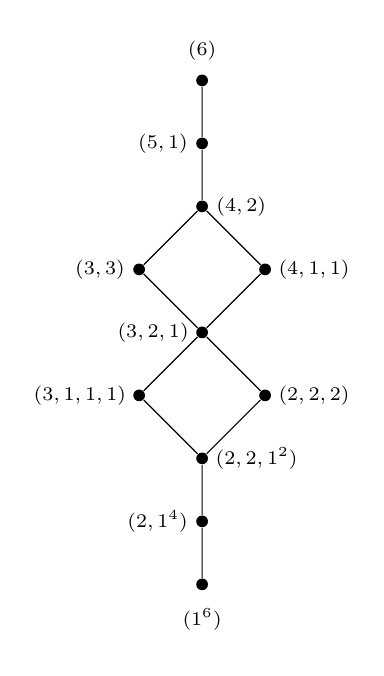
\begin{tikzpicture}[every node/.style={circle, fill, inner sep=1.5pt},scale=0.8]
\node[label=above:{\scriptsize$(6)$}] (6) at (0,8) {};
\node[label=left:{\scriptsize$(5,1)$}] (51) at (0,7) {};
\node[label=right:{\scriptsize$(4,2)$}] (42) at (0,6) {};
\node[label=left:{\scriptsize$(3,3)$}] (33) at (-1,5) {};
\node[label=right:{\scriptsize$(4,1,1)$}] (411) at (1,5) {};
\node[label=left:{\scriptsize$(3,2,1)$}] (321) at (0,4) {};
\node[label=right:{\scriptsize$(2,2,2)$}] (222) at (1,3) {};
\node[label=left:{\scriptsize$(3,1,1,1)$}] (3111) at (-1,3) {};
\node[label=right:{\scriptsize$(2,2,1^2)$}] (2211) at (0,2) {};
\node[label=left:{\scriptsize$(2,1^4)$}] (21111) at (0,1) {};
\node[label=below:{\scriptsize$(1^6)$}] (111111) at (0,0) {};

\draw (111111)--(21111)--(2211)--(222)--(321)--(411)--(42)--(51)--(6);
\draw (2211)--(3111)--(321);
\draw (321)--(33)--(42);
\end{tikzpicture}
\] 

\begin{definition}
    \label{def:lex_order}
    Για δυο (διαφορετικές) διαμερίσεις $\lambda$ και $\mu$ του $n$, γράφουμε $\lambda >_\lex \mu$ και λέμε ότι η $\lambda$ είναι \defn{λεξικογραφικά μεγαλύτερη} της $\mu$ αν για το μικρότερο $i \ge 1$ για το οποίο $\lambda_i \neq \mu_i$ ισχύει ότι $\lambda_i > \mu_i$.
\end{definition}

Το ζεύγος $(\Par(n),<_\lex)$ είναι μια ολική διάταξη η οποία επεκτείνει\footnote{Μια ολική διάταξη η οποία επεκτείνει μια μερική διάταξη ονομάζεται \emph{γραμμική επέκταση} (linear extension).} την διάταξη κυριαρχίας, δηλαδή 
\[
\lambda \triangleright \mu \ \then \ \lambda >_\lex \mu,
\]
για κάθε δυο διαμερίσεις $\lambda, \mu \in \Par(n)$ (γιατί;). Στο παράδειγμα, για $n=6$ έχουμε 
\[
(1^6) <_\lex \cdots <_\lex (2,2,2) <_\lex (3,1^3) <_\lex (3,2,1) <_\lex (3,3) <_\lex (4,1,1) <_\lex \cdots <_\lex (6).
\]

Η Πρόταση~\ref{prop:dominance_lemma} μας πληροφορεί ότι αν $T$ και $Q$ είναι ταμπλώ σχήματος $\lambda$ και $\mu$ τέτοια ώστε $\nabla_T^-[Q] \neq 0$, τότε $\lambda \tge \mu$. Αυτό έχει ως συνέπεια το εξής.

\begin{proposition}
    \label{prop:hom_specht_young}
    Έστω $\lambda, \mu \vdash n$. Αν $\varphi \in \Hom_{\fS_n}(\sS^\lambda,\rmM^\mu)$ είναι μη μηδενική, τότε $\lambda \tge \mu$. Ειδικότερα, αν $\lambda = \mu$, τότε $\varphi = c\,\rmid$, για κάποιο $c \in \CC$.
\end{proposition}

\begin{proof}[Απόδειξη]
    Αν $\varphi \in \Hom_{\fS_n}(\sS^\lambda,\rmM^\mu)$ είναι μη μηδενική, τότε υπάρχει ταμπλώ $T$ σχήματος $\lambda$ τέτοιο ώστε $\varphi(\bfe_T) \neq 0$. Επεκτείνουμε την $\varphi$ σε ολόκληρο το $\rmM^\lambda = \sS^\lambda \oplus (\sS^\lambda)^\perp$, θέτοντας $\varphi((\sS^\lambda)^\perp) = 0$. Έτσι, μπορούμε να γράψουμε 
    \[
    \varphi([T]) = c_1[Q_1] + c_2[Q_2] + \cdots + c_k[Q_k],
    \]
    για κάποια ταμπλοειδή $[Q_i]$ σχήματος $\mu$ και κάποια $c_i \in \CC$. Συνεπώς, 
    \begin{align*}
    \varphi(\bfe_T) 
    &= \varphi(\nabla_T^-[T]) \\
    &= \nabla_T^-\varphi([T]) \\
    &= \nabla_T^-\left(c_1[Q_1] + c_2[Q_2] + \cdots + c_k[Q_k]\right) \\
    &= c_1\nabla_T^-[Q_1] + c_2\nabla_T^-[Q_2] + \cdots + c_k\nabla_T^-[Q_k],
    \end{align*}
    όπου η δεύτερη ισότητα έπεται από το ότι η $\varphi$ είναι $\fS_n$-ομομορφισμός. Επειδή $\varphi(\bfe_T) \neq 0$, υπάρχει κάποιο $1 \le i \le k$, για το οποίο $c_i\nabla_T^-[Q_i] \neq 0$ και κατά συνέπεια $\nabla_T^-[Q_i] \neq 0$. Από την συζήτηση πριν την Πρόταση \ref{prop:hom_specht_young} έπεται ότι $\lambda \tge \mu$.

    Αν $\lambda = \mu$, τότε από το Λήμμα 11.7 (4) έπεται ότι 
    \[
    \varphi(\bfe_T) = c_1\nabla_T^-[Q_1] + c_2\nabla_T^-[Q_2] + \cdots + c_k\nabla_T^-[Q_k] = c\,\bfe_T
    \]
    για κάποιο $c \in \CC$. Το ζητούμενο έπεται από την κυκλικότητα του $\sS^\lambda$.
\end{proof}

\begin{theorem}
    \label{thm:specht_irreducible_complete_set}
    Το 
    \[
    \{\sS^\lambda : \lambda \vdash n\}
    \]
    αποτελεί ένα σύνολο αν δύο μη ισόμορφων ανάγωγων $\fS_n$-προτύπων.
\end{theorem}

\begin{proof}[Απόδειξη]
    Από το Πόρισμα 11.6 γνωρίζουμε ότι κάθε πρότυπο Specht είναι ανάγωγο. Επίσης, αν $\lambda \neq \mu$, τότε προφανώς $\sS^\lambda \ncong_{\fS_n} \sS^\mu$. Συνεπώς, αρκεί να αποδείξουμε ότι αν $\sS^\lambda \cong_{\fS_n} \sS^\mu$, τότε $\lambda = \mu$. Αυτό είναι άμεση συνέπεια της Πρότασης \ref{prop:hom_specht_young}.

    Πράγματι, αν $\sS^\lambda \cong_{\fS_n} \sS^\mu$, τότε $\Hom_{\fS_n}(\sS^\lambda,\sS^\mu) \neq \{0\}$ και γι αυτό $\lambda \tge \mu$. Επίσης, $\Hom_{\fS_n}(\sS^\mu, \sS^\lambda) \neq \{0\}$ και γι αυτό $\mu \tge \lambda$. Άρα, $\lambda = \mu$.
\end{proof}

Το Θεώρημα \ref{thm:specht_irreducible_complete_set} μας πληροφορεί ότι η ολική διάταξη του $\Par(n)$ που ψάχναμε είναι η λεξικογραφική διάταξη (ή, πιο σωστά, η \textquote{ανάποδή} της). Έτσι ολοκληρώνεται το πρόγραμμα που ξεκινήσαμε στην αρχή της παραγράφου.
\begin{corollary}
    Για $\mu \vdash n$, η ισοτυπική διάσπαση του προτύπου Young δίνεται από 
    \begin{equation}
        \label{eq:young_rule}
        \rmM^\mu \cong_{\fS_n} \bigoplus_{\lambda \ge_{\lex} \mu} \left(\sS^\lambda\right)^{m_{\lambda\mu}},
    \end{equation}
    όπου $m_{\lambda\mu} \in \NN$ με $m_{\lambda\lambda} = 1$.
\end{corollary}

\begin{proof}[Απόδειξη]
    Από το Θεώρημα~\ref{thm:specht_irreducible_complete_set} έπεται ότι 
    \[
    \rmM^\mu \cong_{\fS_n} \bigoplus_{\lambda \vdash n} \left(\sS^\lambda\right)^{m_{\lambda\mu}},
    \]
    όπου 
    \[
    m_{\lambda\mu} = \dim\left(\Hom_{\fS_n}(\sS^\lambda,\rmM^\mu)\right),
    \]
    από το Λήμμα 3.6. Το ζητούμενο έπεται από την Πρόταση \ref{prop:hom_specht_young}.
\end{proof}

Οι αριθμοί $m_{\lambda\mu}$ που εμφανίζονται στην Ταυτότητα \eqref{eq:young_rule} ονομάζονται \defn{αριθμοί Kostka}. Είναι φυσικό να ρωτήσει κανείς τι απαριθμούν. Αργότερα, θα δούμε μια συνδυαστική τους ερμηνεία. Για την ώρα, χρησιμοποιώντας κανείς τον πίνακα χαρακτήρων της $\fS_4$ μπορεί να υπολογίσει τον πίνακα $(m_{\lambda\mu})_{\lambda,\mu \, \vdash 4}$, ο οποίος είναι 
\[
\renewcommand{\arraystretch}{1.2}
\begin{array}{c|ccccc}
              & (4) & (3,1) & (2,2) & (2,1,1) & (1,1,1,1) \\\hline
    (4)       & 1   & 0     & 0     & 0       & 0 \\
    (3,1)     & 1   & 1     & 0     & 0       & 0 \\
    (2,2)     & 1   & 2     & 1     & 0       & 0 \\
    (2,1,1)   & 1   & 2     & 1     & 1       & 0 \\
    (1,1,1,1) & 1   & 3     & 2     & 3       & 1 \\
\end{array}.
\]
Ποιός είναι ο αντίστοιχος πίνακας για $n=5$;
\end{document}